\section{Approach}
In this section, we introduce the proposed framework for multiple MDD, including symptom identification and a two-stream Psychiatric Experts Model. 
First, we give the definition of multiple MDD here. Given the posting history of a user with N posts: $\{p_1, p_2, ..., p_N\}$, and a list of $M$ potential mental diseases, the goal is to detect which disease(s) in the $M$ candidates does the user suffer from. Typically, this can be accomplished by training $M$ separate models for each disease. Here, we further propose a novel method that leverage a single model to effectively learn the distinctions and commonality among diseases for a better overall performance on all diseases. 
% The symptom identification phase can generate the symptom stream and utilize a symptom-based risky post screening to select posts for the risky post stream.
% \KZ{Where do we make the problem definition of multiple MDD? I think this should be done properly, because what we are doing is given a history of user posts, predict if the user has any or some of the $K$ diseases. Previously, the single MDD is only for a particular disease. It would appear possible to straight-forwardly adapt a single MDD model to a multi-disease MDD problem (e.g., u can train K models and run them each on the same input to get K results), but we have to argue that this is not so simple.}

\subsection{Symptom-based Risky Posts Screening}
\label{sec:symp_screen}
Traditional MDD method processes every single post equally overlooking the fact that not every post from a patient reveals useful information for detection. To facilitate the MDD model performance, as well as provide explainable diagnosis basis, we screen risky posts first, in particular with disease-dependent symptom information, and use the selected posts for multiple disease detection. 

Inspired by clinical diagnosis procedures, we assume that posts reflecting \textit{symptoms} of mental disorders suggest higher risks. Since healthy individuals rarely produce symptom-related content, posts with symptom indications could better separate patients from control users. Hence, unlike the prior heuristic methods discussed in 
\secref{sec:intro}, we implement a screening method based on the symptom features extracted by a supervised symptom identification model\footnote{The code and data of the symptom identification model can be found at \url{https://github.com/blmoistawinde/EMNLP22-PsySym}} \cite{Zhang2022SymptomIF}.
This model can identify 38 symptom classes from 7 mental diseases with a Mental BERT-based encoder \cite{ji2021mentalbert} and a linear classifier. It is trained on a large-scale, multi-disease annotated symptom identification dataset, based on the globally-accredited diagnostic criteria from Diagnostic and Statistical Manual of Mental Disorders (DSM-5)~\cite{american2013diagnostic}. 

The symptom feature of each post is a 38-dimensional vector, where each dimension is the predicted probability of a certain symptom~\footnote{These symptoms (e.g., \textit{anxious mood, sleep disturbance, poor memory}) are carefully extracted from DSM-5, so that there is as little semantic overlap as possible 
between them. We list all the symptoms in \tabref{tab:symp_id} (Appendix~\ref{apd:symps}).}.
We can then estimate the \textit{risky score} of a post with the \textit{sum} of predicted probability among all symptoms. The top $K$ posts with highest risky score among a user's whole posting history (containing $N$ posts) will be selected as his/her risky posts. In practice, we set $K \ll N$, so the reduced input size enables high efficiency even with BERT-based language models in the following disease detection phase. Moreover, the symptom extracted by a supervised model is also more reliable to select risky posts than heuristic approaches, and we will show this in the experiments (\secref{sec:ablation}).

\subsection{Two-Stream Psychiatric Experts Model}
\label{sec:PsyEx_model}

Although MDD can be formulated as a typical text classification problem, traditional model structures are not appropriate for our multiple mental disease detection task for two primary reasons. On the one hand, employing a single user representation to detect all diseases would overlook the explicit differences between them. Conversely, if each disease is detected separately, the neglect of shared symptoms across these diseases will also adversely affect the overall performance.
% \KZ{Why single user representation can't catch different diseases?  I don't see the necessary logic here.}
\begin{figure}[th]
    \centering
    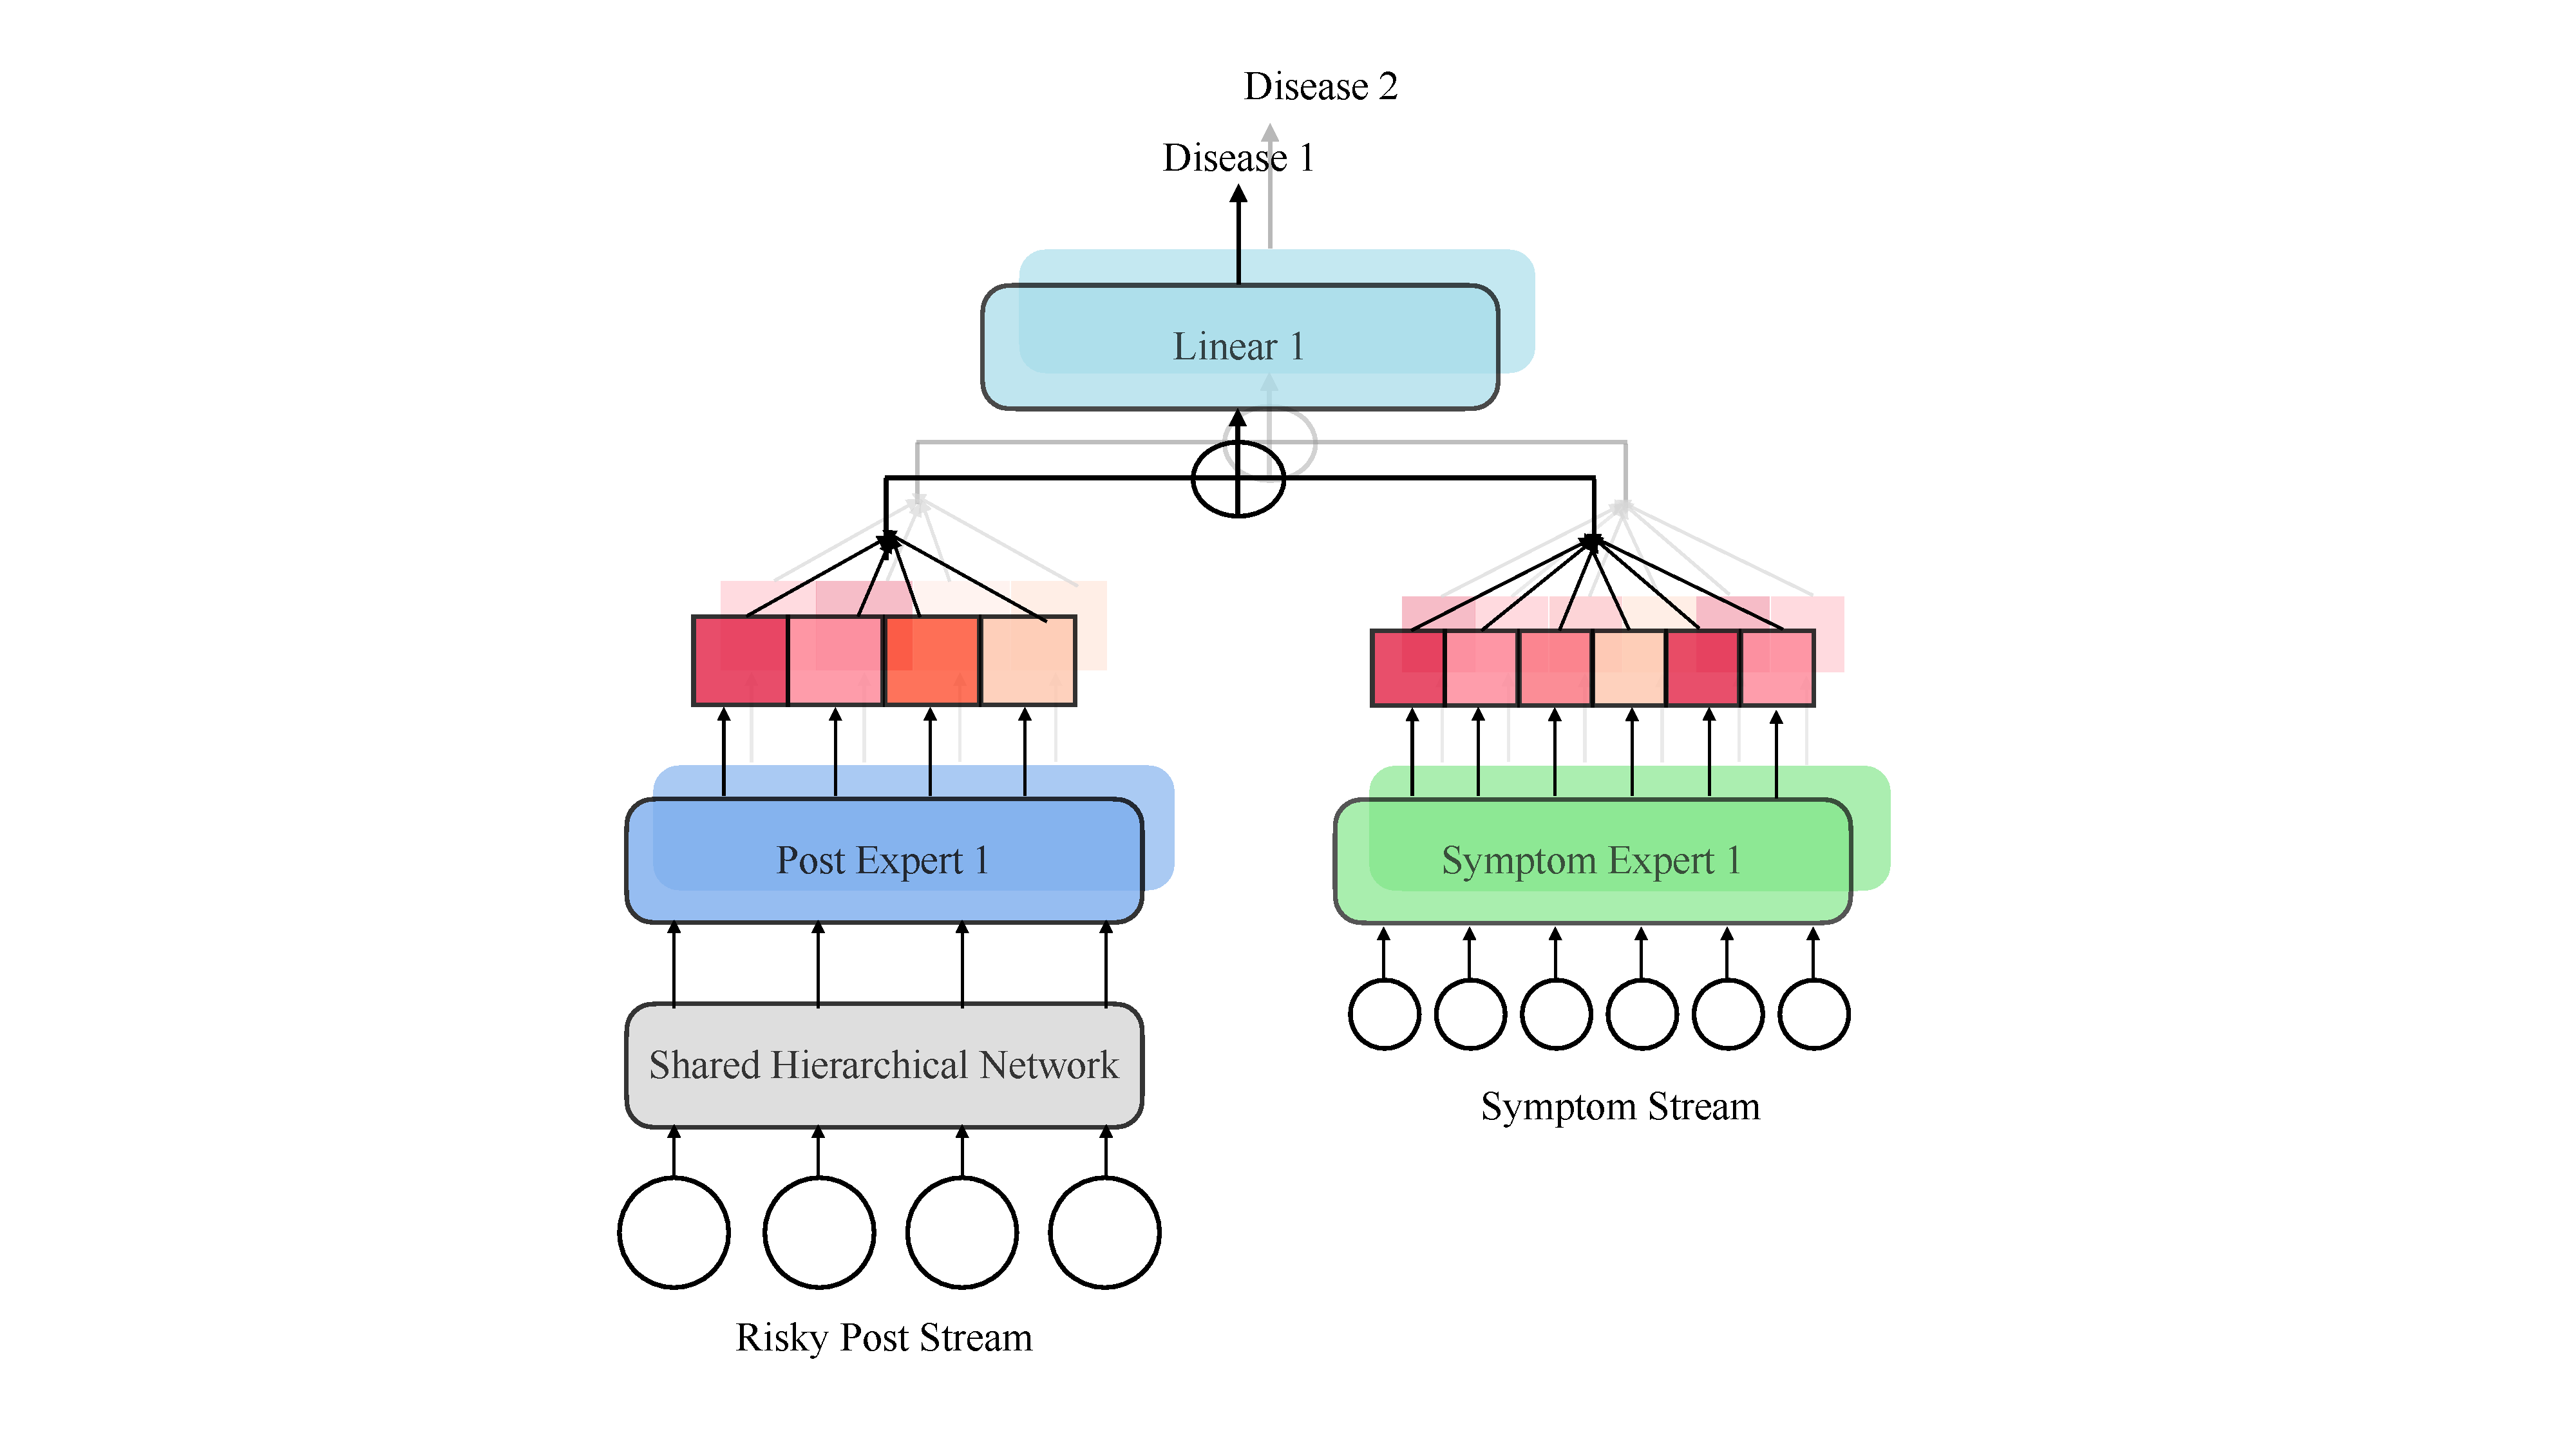
\includegraphics[width=0.9\columnwidth]{figures/model_arch.pdf}
    \caption{Illustration of the proposed model architecture, with 2 disease-specific experts on top of a shared network. Darkness of red
square indicates attention strength, which is different for each disease.}
    \label{fig:model_arch}
\end{figure}


To alleviate this problem, we propose a Two-Stream Psychiatric Experts Model
(See \figref{fig:model_arch}), which can detect all the mental diseases simultaneously through multi-task learning while still capturing the nuances among them. 
It takes \textit{risky post stream} and \textit{symptom stream} obtained in symptom identification phase as input to combine the advantages of both modalities. 

\paragraph{Risky Post Stream Model} The risky post stream ``cherry-picks'' $K$ 
posts with highest symptom probability, providing more strong and concentrated signals of mental diseases. 
To better explore these signals and distinguish among multiple diseases, 
the model consists of two components: a single \textbf{shared hierarchical network} and \textbf{$D$ disease-specific post experts}.  

In the shared part, we draw on the structure of Hierarchical Attention Network (HAN) \cite{yang2016hierarchical} with post and user-level encoder to make better use of the sequential structure of the posts.
We employ a pre-trained BERT model as the post encoder. For 
words $\{w_1, w_2, ..., w_L \}$ in a post, the post representation $p$ is,
\begin{equation}
    p = BERT_{[CLS]}(w_1, w_2, ..., w_L)
\end{equation}
The user-level encoder utilizes a transformer \cite{vaswani2017attention} structure, modeling the relations between these posts $\{p_1, p_2, ..., p_K\}$, and produces updated post representations $\{p'_1, p'_2, ..., p'_K\}$.

In the disease-specific part, each disease $d$ has its own attention layer to get different attention distributions on the same post sequence. 
As such, these $D$ attention layers can be considered as feature selectors from the shared network \citep{Liu2019EndToEndML}. 
Then we perform a weighted sum of the post representations according to attention score to get the distinctive user representations $u_d$. 
\begin{equation}
    \alpha_{k, d} = \frac{exp(W_d p'_k + b_d)}{\sum_{k'=1}^{K} exp(W_d p'_k + b_d)}
\end{equation}
\begin{equation}
    u_d = \sum_{k=1}^K \alpha_{k, d} p'_k
\end{equation}
where $W_d$ and $b_d$ are both learnable parameters specifically for disease $d$. 

The attention distribution on the post sequence reflects the weight of each post in the final prediction. Therefore, the attention score can offer interpretability of the model decision, which will be further discussed in \secref{sec:interpret}


\paragraph{Symptom Stream Model} 
% \KZ{I think here you want to motivate why we use this separate symptom stream since the text post stream already contain all the info. We need to say that our belief is that symptoms play very important roles in MDD, so they are not only used in post screening, but also in user history representation. Just using the text representation is not enough, because ...}
Symptom feature is critical for MDD, because it equips the detection model with explicit psychiatric knowledge. The symptom stream can be considered as an $N \times 38$ matrix, revealing a user's whole posting history in a lighter way, 
which is able to replenish the incomplete text stream and provide holistic 
information for the detection model.
To better capture the unique features of different diseases, the symptom stream model is totally disease-specific, and its structure is the same as the corresponding part in risky post stream model. Similarly, each disease has its own ``expert'' to get different attention distributions on the same symptom sequence, which is intuitive because each mental disease has its own typical or unique symptoms for diagnosis (e.g., panic fear for Anxiety, intrusion for PTSD). 

Finally, the disease-specific user representation from both stream are concatenated and fed into separate linear layers to get the binary predictions on whether the user suffers from a certain mental disease. 

The whole model is trained with the standard binary cross entropy loss, where the loss of all the tasks are averaged. In the dataset, we usually have patients that are certain for the diagnosis of some diseases but uncertain for others, and we should not assume these diseases to be not existing due to the high comorbidity of diseases. Therefore, we implement \textit{loss masking} as described in \citet{fonseca2020addressing}, 
so that for patients with at least one disease, we do not consider their absent disease labels as negative (i.e., we assign zero weight to exclude them from affecting the training loss). This approach helps alleviate the problem of potentially missing labels. We can get more reliable negative labels from control users who show no signals of mental issues.

% \KZ{I don't understand the following? How do you handle missing labels? Why not use a formula to say this clearly? What about patient with no diseases?}


%myw not focusing on what you did, but first make clear why you did it. You introduced the framework of two stages but didn't mention why you did it like this. For example, to better disentangle multiple diseases and promote detection efficiency, we first involve symptoms to screen risky posts...
%myw maybe start like: Traditional MDD method processes every single post equally overlooking the fact that not every post from a patient reveals useful information for detection. To facilitate... We screen risky posts first, in particular with disease-dependent symptom information...for multidple disease detection. 
% To obtain a high risky score in \textit{Sum} pooling, a post must have more symptoms with relatively high probability, while in \textit{Max} pooling, only one high enough probability is needed. 
% \MYW{Is there anything novel about the screening process? If not, consider moving it into experiments part and take it as a data preprocessing method, then you experimented two different pooling methods. If you consider using PsySym as a new method to screen risky posts, make it more obvious. "Different from previous risky screening method, we implement.."}




